\chapter{Enabling long-term structural changes. Dynamic connectomes.}
\label{ch:dynamic_connectome}

In this section, we increase the complexity of the system by implementing a mechanism for long-term structural changes, enabling learning. These lasting changes are crucial for any environmental adaptation we want our system to do. This also serves as an alternative strategy for coping with the device parameter variability.

In neural network models, following the biological evidence, these structural changes are primarily implemented with permanent changes of connection efficacies, or, for \ac{SNN}s, synaptic weight updates. Indeed, the principle of functional learning through inter-neuron connection weight updates in biological networks has been widely demonstrated \emph{in vivo} as well as \emph{in vitro} through synaptic growth, transformations and pruning~\cite{George18}.
Moreover, the way these weights are updated plays a fundamental role in what function the network will or will not be able to learn. Thus, the choice of the appropriate learning rule determines the possibility of capturing and extracting the relevant features in the input stream fed to the network. At the same time, while mathematically we can engineer a multitude of options, both biological and hardware constraints help us limit our variety of solutions. While ANNs tend to employ (to the great success~\cite{Sejnowski20}) global weight update strategies such as output error backpropagation, where individual weight increments can only be calculated synchronously and with access to the entire weight matrix at once, the biological synapse conductance is largely driven by the correlated pre- and postsynaptic activity, only vaguely depending on the global network state. On the hardware side of things, centralized approaches burn a lot of energy gathering centralized information about the entire system to make the update step. Biology tends to save the limited resources as much as possible, and local information processing is a direct result of that.

By design, the DYNAP-SE1 chip does not have any synaptic plasticity. However, we can exploit the nature of its asynchronous routing mechanism that does not interrupt the spiking dynamics, to perform some dynamic connectivity changes.

In this chapter, I introduce a hardware-constrained local spike-based so-called ``neo-Hebbian''~\cite{Gerstner_etal18} reward-gated STDP learning rule and additional regulatory mechanisms fitting the considerations above and show its implementation for the \ac{DYNAP}-SE1 chip. The learning rule fits the chip's routing architecture as, while being spike-based, it only applies cumulative updates. Given the low precision of the weight on the chip, a heavy stochastic quantization method is applied, which also introduces a computational advantage serving as a built-in exploration mechanism. Since the updates are calculated externally to the chip, we argue that such approach could be used for testing any alternative learning rules as long as the meet the criteria of sparsity of the weights and cumulative non-frequent updates.

This resulting learning framework is then applied in conjunction with the static network structures introduced in the previous chapter to demonstrate biologically plausible examples of learning in an on-chip network of spiking neurons (see Chapter~\ref{ch:EXAMPLES}).


\section{Revisiting neuromorphic routing. Weight multiplexing. Chip-in-the-loop discussion.}

To find the matching learning rule applicable to our hardware case, we need to revisit the connectivity constraints of our chip.

On DYNAP-SE1 chip, communication between hardware spiking neurons is implemented via the \ac{AER} protocol ~\cite{Sivilotti91, Deiss_etal94, Boahen00}: the system of asynchronous hierarchical digital routers transfers an ``event'' - a single packet of data containing the timestamp of the occurrence of the event (spike), and the address of the source neuron that emitted that spike~\cite{Moradi_etal18}.
The \ac{AER} event is registered by the router at the moment of occurrence at the neuron and is broadcast to all synapse circuits of all neurons of the target chip(s). The routing information is stored in two parts: (i) the emitting neuron circuit has a dedicated \ac{SRAM} cell that defines which target \emph{chips} the event is broadcast to; (ii) every neuron has 64 10-bit \ac{CAM} registers defining spikes from which neurons should be accepted as source. In case of the matching source neuron ID (identical to the one written in the CAM cell), the chain of the dedicated pulse generator (PG) and the pulse extender (PE) blocks induces a current in the respective analog DPI synapse circuit (illustrated in Figure~\ref{fig:dynapse_AER_block}).

\begin{figure}[h]
  \centering
    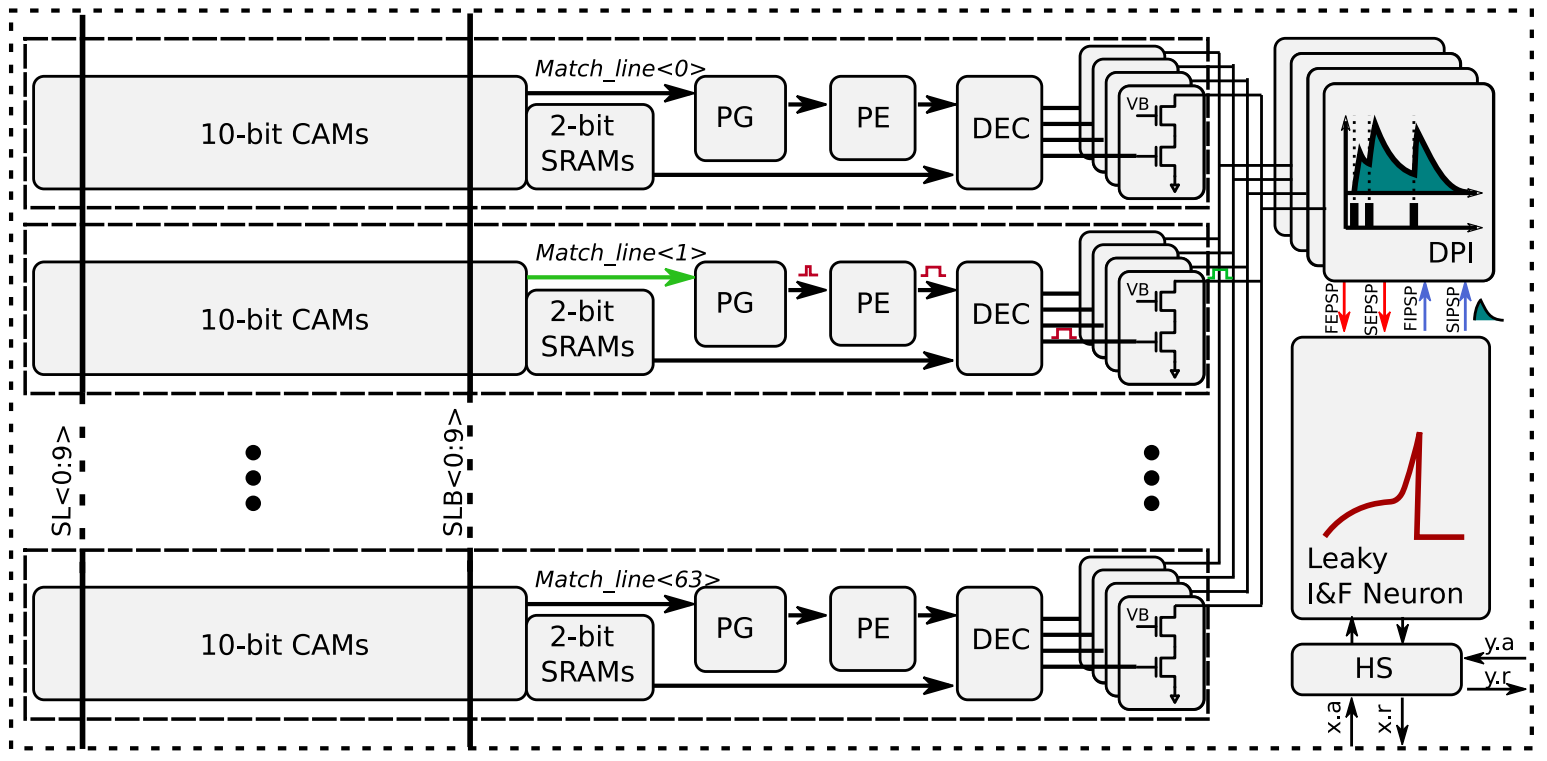
\includegraphics[width=.9\textwidth]{img/chapter4/dynapse_neuron_block_diagram.png}
    \caption[AER processing block of one neuron of the DYNAP-SE1 core]{Neuronal AER processing block, Figure 9 in~\cite{Moradi_etal18}, showing the chain of circuits generating a PSP upon receiving the matching source AER event.}
  \label{fig:dynapse_AER_block}
\end{figure}


The central principle we need to note here is what happens when multiple CAM cells are programmed to hold the same source neuron address. The respective PG-PE chains will be triggered simultaneously, generating fully aligned EPSPs/IPSPs on the same neuron, depending on the synapse type set in the CAM cell. And if the selected types are identical, it will indeed be the very same physical analog synapse circuit processing the same input event multiple times. Since these chains act independently, the resulting effect on the DPI synaptic circuit is additive, which we can use for multiplexing (i.e. selectively multiplying, and thus controlling) the individual functional weights (efficacies) between the pairs of neurons while the analog continuous \emph{weight biases} are still shared between all same-type synapses of the core.

\begin{figure}[b!]
  \centering
    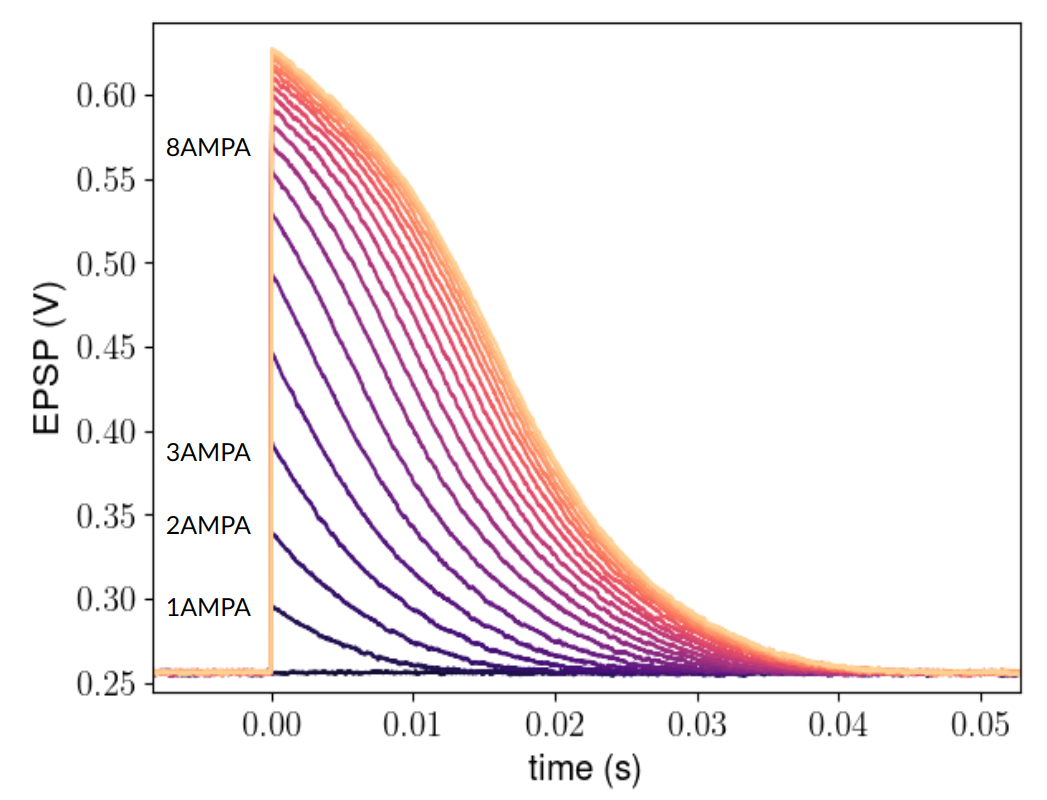
\includegraphics[width=.7\textwidth]{img/chapter4/CAM_multiplexing.png}
    \caption[Multiplexing CAMs for quantized weight control]{Automated and time-synchronized measurement of an AMPA EPSP generated by a single input spike with multiple CAM cells listening to the same input neuron, effectively creating duplicate parallel connections between the two neurons. The measurement shows that, at first, the amplitude of the first peak increases linearly with the number of parallel AMPA connections but then saturates at higher values.}
  \label{fig:CAM_multiplexing}
\end{figure}

To verify and characterize this mechanism, we look at the EPSP shape when measuring the neuron membrane voltage, as the direct observation of synaptic behaviour is unavailable on the DYNAP-SE1 chip. To observe the approximate shape of the EPSP, we once again set the neuron circuit leak to the maximum value to eliminate any synaptic input integration. 


Figure~\ref{fig:CAM_multiplexing} shows a measurement from a postsynaptic neuron receiving a spike through multiple CAM cells listening to the same input neuron, routed through an AMPA DPI synapse. The pulses arriving through parallel CAM blocks are summed up at the synapse circuit, adding to the amplitude of the resulting EPSP. The increments of the EPSP amplitude are dependent on the synapse circuit weight bias, while the DPI threshold bias controls the maximum amplitude that the EPSP would never exceed. At first, the EPSP amplitude increments are constant (i.e. the PSP amplitude scalers linearly), but are then reduced and eventually saturate with more than 8-10 parallel connections.


This gives us some understanding of how rough is our control over individual weights on the chip (i.e. 3-bit weights effectively). On top of this, since each neuron has only 64 CAM cells in total, using multiple of them takes away from the total number of possible inputs of the neuron. Indeed, these multi-CAM profiles are still different for different physical DPI circuits due to variability through mismatch.

%\subsection{Global vs local updates, in the loop.}

%\dz{Single-weight vs batched connectivity matrix updates, show why batched updates are favoured for our case.}
%\bigskip
%\dz{Fusi learning rule, Machens learning rule and applicability.}
%\bigskip
%\dz{Mention transfer learning, He Xu's 2019 Capocaccia with the first chip in the loop attempt.}
%\bigskip



\subsection{Weight quantization}

Several extra steps must be taken to perform the weight changes on the DYNAP-SE1 chip. The weight matrix on the chip can be reprogrammed without interrupting the neural activity; however, no learning rules can be enabled on the chip itself. Moreover, the true weight value of one synapse created between the two neurons is determined by the analog bias shared by design of chip layout between all synapses of this type in the given core. As shown above with the EPSP scaling measurement, individual \textit{effective weights} can be set by creating multiple \textit{parallel} synapses between the pair of neurons, which results in their low, or quantized, precision.\\

\begin{figure}[b!]
  \centering
    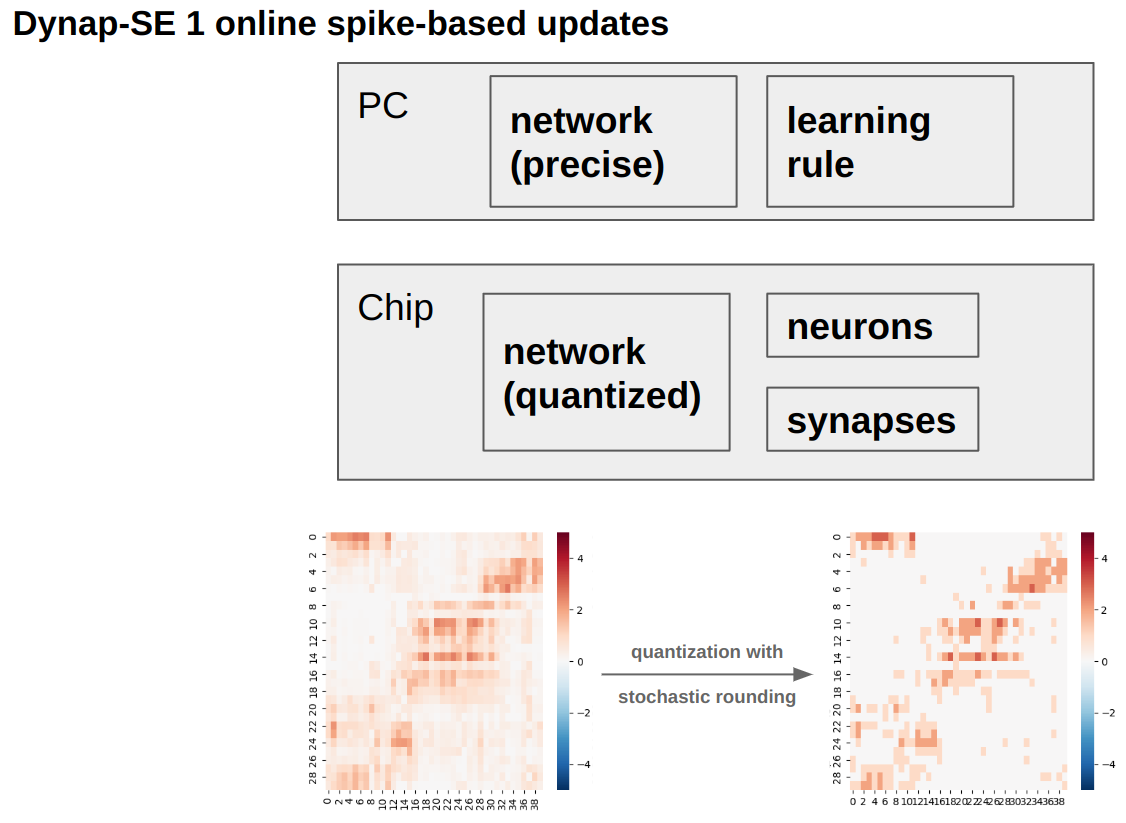
\includegraphics[width=.7\textwidth]{img/chapter4/chip_in_the_loop_logic.png}
    \caption[Chip in the loop with storage of the precise and quantized versions of weight matrices.]{Chip in the loop weight matrix update logic illustration, with the precise and quantized matrices on the lower panel. The chip router configuration uses the quantized matrix, and thatis the matrix that the physical neurons of the chip interact through. The algorithmic overhead on the PC retrieves the spikes from the chip in a fast loop and updates the precise floating-point weights based on any arbitrary weight update mechanism. The precise matrix then is stochastically quantized when applied to the chip.}
  \label{fig:weight_quantization}
\end{figure}

We implemented an additional quantization step every time the weight matrix was updated and applied to the chip. Inspired by stochastic rounding in fixed precision calculations~\cite{Hopkins_etal20} and an example for limited weight precision ANN training~\cite{Gupta_etal15}, we implemented a similar algorithm for our case.\\

The idea is simple. We introduce the quantization step $\Delta_q$ as a parameter defining the precision of our effective weights. Then we take a weight $w^{ij}_p \in W_p$ and divide it by $\Delta_q$. The two rounding options would be lower $\lfloor \frac{w^{ij}_p}{\Delta_q}\rfloor$ and the higher $\lceil \frac{w^{ij}_p}{\Delta_q}\rceil$ nearest integers values. We round up or down stochastically, by generating a random number between 0 and 1, and comparing it to the fractional part $\{\frac{w^{ij}_p}{\Delta_q}\}$ as a probability to round \emph{up}.

In our framework, we kept two versions of the plastic weight matrix at all times: a matrix of precise weights $W_p \in \mathbb{Q}^{m \times n}$, used for all weight calculations of the given learning rule, and a quantized integer matrix $W_q \in \mathbb{Z}^{m \times n}$, applied to the chip. Conversion from $W_p$ to $W_q$ was done every time the hardware matrix update was required by the learning rule (concept illustrated in Figure~\ref{fig:weight_quantization}).


An additional constraint for the quantization procedure is, of course, the fan-in limit of 64 CAM slots for every neuron. Since we never impose any sparsity on the precise matrix $W_p$, it has to be applied during the quantization procedure. The two obvious strategies are the ``greedy'', when the available CAM slots are attributed to the highest weights first, or the uniform, where the ``ideal'' quantized matrix is uniformly downsampled until it fits (see Figure~\ref{fig:weight_quantization_strategies} for illustration). The figure also illustrates the importance of choice of the quantization step $\Delta_q$, as the increment of the EPSP with each $\Delta_q$ step is equal to the values set by the analog weight bias.

Thus, the full weight update procedure upon the arrival at time on-chip matrix update signal was the following:
\begin{itemize}
    \item New values of precise weights $W_p^{new}$ were calculated based on the old weights $W_p^{old}$ and the updated given by Equation~\ref{eq:reward} using the current values of eligibility traces.
    \item The precise matrix was then $W_p^{new}$ quantized using procedure shown in Figure~\ref{fig:weight_quantization}, creating a matrix of integer values $W_q^{new}$.
    \item The new quantized matrix $W_q^{new}$ was applied to the DYNAP-SE1 chip, creating the corresponding number of logical synapses for each pair of pre- post- neurons.
\end{itemize}

\begin{figure}[t!]
\begin{subfigure}{.4\textwidth}
\centering
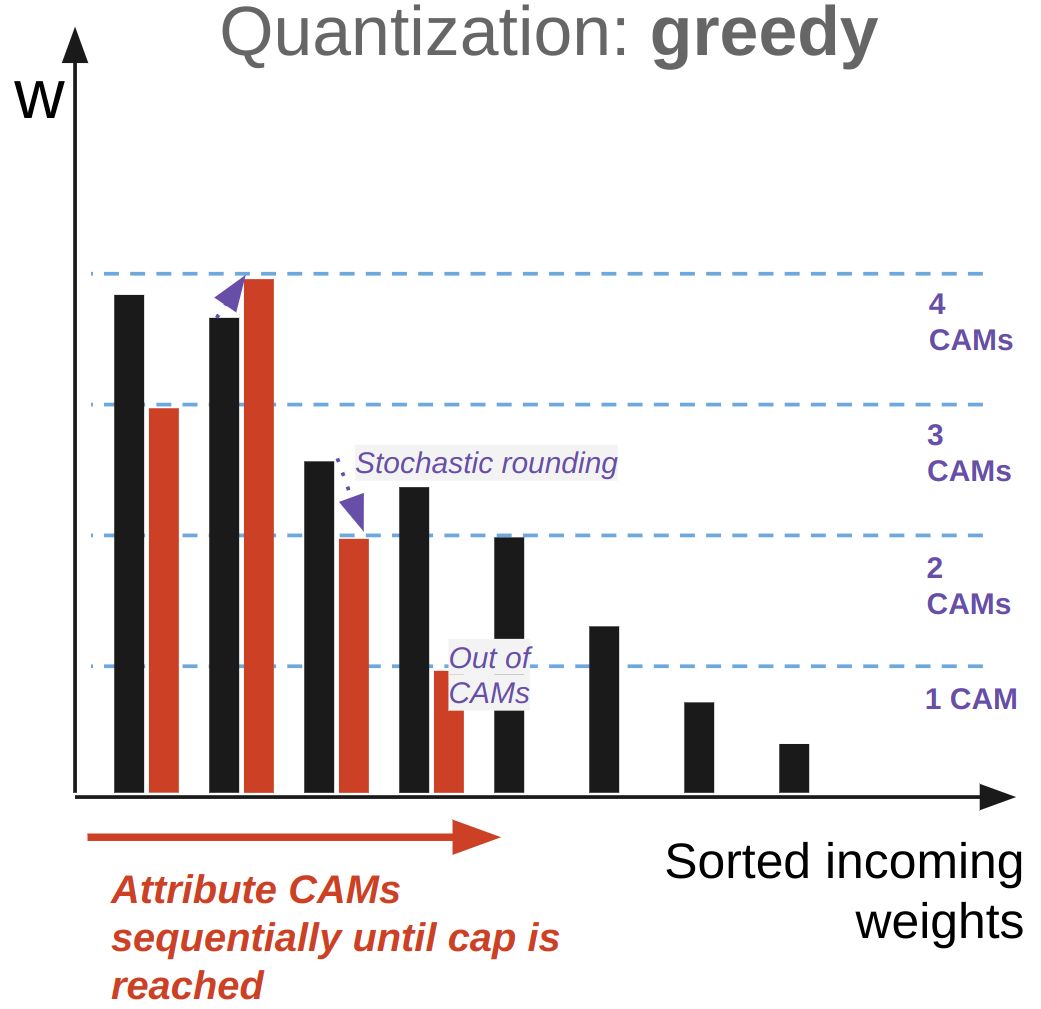
\includegraphics[width=\linewidth]{img/chapter4/quantization_greedy.png}
\caption{}
\label{fig:quantization_greedy}
\end{subfigure}
\hfill
\begin{subfigure}{.44\textwidth}
\centering
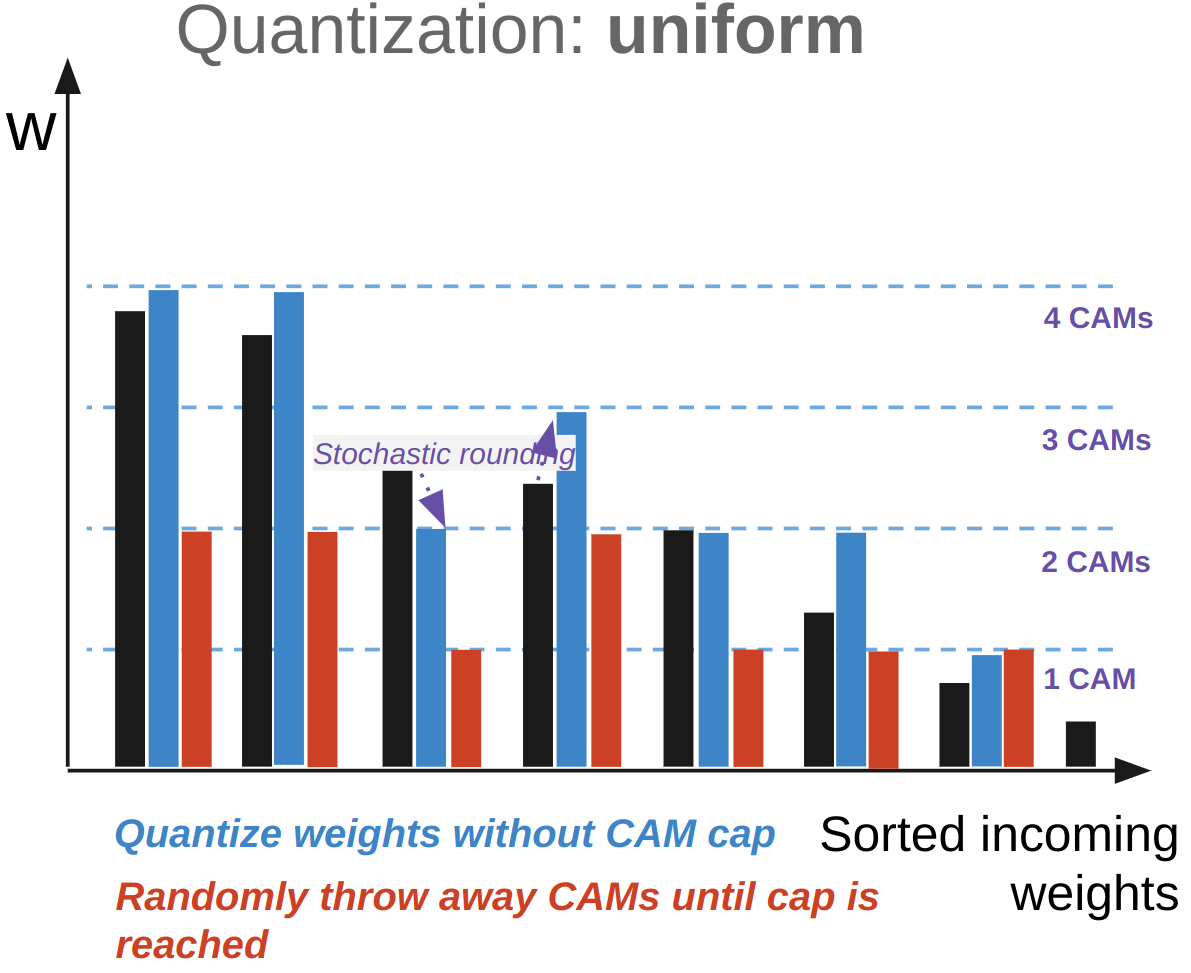
\includegraphics[width=\linewidth]{img/chapter4/quantization_uniform.png}
\caption{}
\label{fig:quantization_uniform}
\end{subfigure}
\caption[Weight quantization strategies]{Weight quantization strategies applied to sorted input weights of a neuron (each black bar represents the value of the weight, decreasing along the X-axis). These precise values are rounded to the integer levels corresponding to the multiples of parallel connections that the neuron would receive. The weights are stochastically rounded up or down with probabilities equal to their fractional parts. The constraint of limited total input per neuron is addressed with one of the two strategies: \subref{fig:quantization_greedy} The greedy strategy preserves the greatest weights, so the input slots (CAMs) are attributed to the quantized set of weights until the cap is reached; \subref{fig:quantization_uniform} The uniform strategy aims to preserve the entire matrix shape, scaling down the quantized weights uniformly by randomly decreasing one of the input weights by 1 until the cap is reached.}
\label{fig:weight_quantization_strategies}
\end{figure}

%\section{Upcoming hardware solutions for long-term synaptic changes}

%\dz{Add a review about memristors, ferroelectric synapses, other variable conductance devices. Reference a lot of Yigit's work. Reference Charlotte's work, Thomas' and Melika's work.}


\newpage
\section{Reward-gated STDP as a hardware-friendly local learning rule}
\label{sec:RSTDP}

\subsection{Combining STDP with the reward signal}

Reward-modulated spike-timing dependent plasticity (R-STDP) is a popular biologically derived weight update mechanism that bridges together the single spike timing interaction timescale, that is typical for Hebbian synaptic changes\cite{Bi_Poo98}, with the behavioural timescales by the means of long-relaxating synaptic eligibility traces that store cumulative weight updates given by STDP~\cite{Schultz97, Izhikevich07, Fremaux_Gerstner16}. The eligibility traces model the presence of the third (in addition to pre- and postsynaptic spikes) factor in the form of the dopamine signal, effectively gating the weight changes. It is sometimes called neo-Hebbian. R-STDP has been shown to be effective for both more classical feedforward SNN training~\cite{Mozafari_etal18} and biological behavioural experiments, especially where loss-function gradients do not apply~\cite{Izhikevich07,Vasilaki09,Gerstner_etal18}.

In this section, we show how the dynamic routing architecture of the DYNAP-SE1 chip fits this cumulative update property.

%\dz{Add references from the Spinnaker and Brainscales RSTDP implementations}\\

%\dz{TAKEN FROM SPINNAKER PAPER, NEEDS REWRITING OR REFERENCING: The reward mechanism in R-STDP is biologically inspired: the phasic activity of dopamine neurons in the brain was found to encode expected reward (Schultz et al., 1997; Hollerman and Schultz, 1998; Bayer and Glimcher, 2005) and dopamine concentration modulates STDP (Pawlak and Kerr, 2008; Edelmann and Lessmann, 2011; Brzosko et al., 2015). R-STDP and similar reward-modulated Hebbian learning rules have been used to solve a variety of learning tasks in simulations, such as reproducing temporal spike patterns and spatio-temporal trajectories (Farries and Fairhall, 2007; Vasilaki et al., 2009; Frémaux et al., 2010), reproducing the results of classical conditioning (Izhikevich, 2007), making a recurrent neural network exhibit specific periodic activity and working-memory properties (Hoerzer et al., 2014) and reproducing the seminal biofeedback experiment by Fetz and Baker (Fetz and Baker, 1973; Legenstein et al., 2008). Compared to classic unsupervised STDP, using R-STDP was shown to improve the performance of a spiking convolutional neural network tasked with visual categorization (Mozafari et al., 2018a,b). In contrast to other learning rules in reinforcement learning, R-STDP is not derived using gradient descent on a loss function; rather, it is motivated heuristically (Frémaux and Gerstner, 2015), the idea being to multiplicatively modulate STDP using a reward term. }

%\dz{Gütig, R., and Sompolinsky, H. (2006). The tempotron: a neuron that learns spike timing-based decisions. Nat. Neurosci. 9, 420–428. \cite{Gutig_Sompolinsky06}}

Unlike the hardware neuron equations discussed in Chapter~\ref{ch:introduction_to_hardware} that are slightly different to the original mathematic model, the equations used for plasticity are not changing in the implementation as they are solved digitally (for this given chip). The core learning algorithm used is the triplet Spike-Time-Dependent-Plasticity (STDP)~\cite{Pfister_Gerstner06}. STDP is a spike-based variant of a biologically plausible local Hebbian learning rule. It is defined by the relative timing of spikes at the pre- and post- neurons and, in the most general formulation, states that the synapse weight is strengthened if the pre- spike occurs before the post- spike and it is weakened in the opposite case. The "triplet" modification accounts for mean firing rates of the neurons as well, adding secondary terms to the weight update equations. The weight change is given by:

\begin{equation}
\Delta w^{+}_{stdp} = r_{1}(t)[A^{+}_{2}+A^{+}_{3}o_{2}(t-\epsilon)],  t=t^{post}
\label{eq:ltp}
\end{equation}
\begin{equation}
\Delta w^{-}_{stdp} = -o_{1}(t)[A^{-}_{2}+A^{-}_{3}r_{2}(t-\epsilon)],  t=t^{pre}
\label{eq:ltd}
\end{equation}

where $A_{i}^{\pm}$ are the weight change amplitudes, and $r_1$, $r_2$, $o_1$ and $o_2$ are exponentially decaying traces increased by 1 upon spiking of the pre- and postsynaptic neurons, respectively (see Figure~\ref{fig:triplet_stdp} for illustration). The $r_2$ and $o_2$ components represent the triplet (or ``rate dependent'') components of the weight update rule (see~\cite{Pfister_Gerstner06} for details).
In our analysis, we follow the suggestion from the authors and use the all-to-all-interactons scheme between the pre- and post-neurons,
meaning that these traces are not clamped to 1. Thus, by integrating the entire history of firing of their respective neurons, each postsynaptic spike is compared to all the previous presynaptic spikes and viceversa.

\begin{figure}[h]
    \centering
    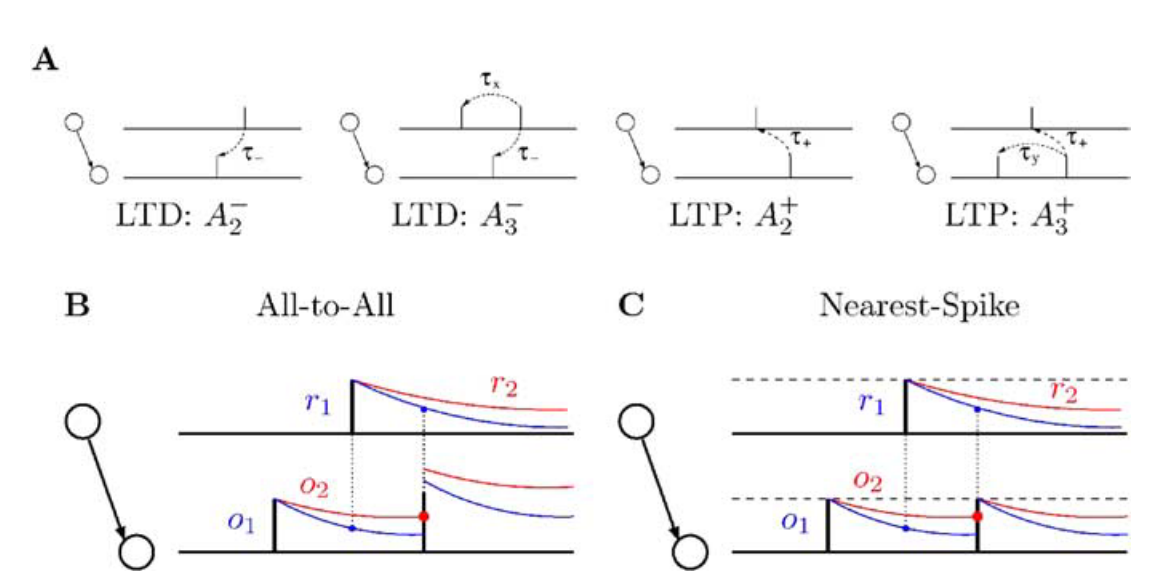
\includegraphics[width=0.8\textwidth]{img/chapter4/pfister2006.png}
    \caption[STDP rule illustration]{Figure 1 from~\cite{Pfister_Gerstner06} showing traces used in the online \ac{tSTDP} implementaion, either allowing the nearest or all-to-all spike interactions to affect the weight change.}
    \label{fig:triplet_stdp}
\end{figure}

To add reward modulation on top of the STDP, we follow the approach of~\cite{Izhikevich07, Gerstner_etal18} combining the triplet STDP algorithm with the delivery of a reward signal. In the paper, the author shows how a reinforcement signal can selectively strengthen the right synapses also seconds after the reward signals has been delivered.
As in standard RL problems, the neurons keep track of the history of the neuron firing and store it in the so-called eligibility trace value. Similarly, we implement such decaying eligibility traces $c(t)$ for every synapse that is affected by STDP updates given by Eqs~\ref{eq:ltp} and~\ref{eq:ltd} instead of the actual weights of synapses:

\begin{equation}
\tau_{c}\frac{dc(t)}{dt} = -c(t) + c_0 \Delta w_{stdp}(t)
\end{equation}

Then, only the eligibility traces are continuously updated with every spike emitted by pre- and postsynaptic neurons, while the weights are updated only when a third factor (the reward) is received:

\begin{equation}
\Delta w(t) = w_0 c(t), t = t_{reward}
\label{eq:reward}
\end{equation}

In some implementations, the weight update is a convolution between the eligibility trace and the reward signal. We decided to keep the reward signal as a delta function for both analysis simplicity and performance reasons.

This approach can be particularly seen as hardware friendly as the weight changes are accumulated by the eligibility traces and are updated in chunks only once in a while (upon the reward arrival), counter to continuous independent weight updates of standard STDP.
%\dz{TBA here: show preliminary behaviour without any regularization here? as just RLSTDP test runs, showing how the activity runs away}


\subsection{Additional regulation mechanism: multiplicative updates, heterosynaptic plasticity}

Since the \ac{tSTDP} learning rule is Hebbian, i.e. positively reinforces spiking correlations, it needs some negative feedback compensation mechanism to avoid overexcitation. That is often done by using asymmetric extended \ac{LTD} time windows, or some constant weight relaxation. In this section, however, we do not touch the R-STDP. Instead, we limit the weight change with two additional ``homeostatic'' rules on top. 

Given quite strict DYNAP-SE1 chip fan-in constraint, an intuitively inspired choice is the limited and/or fixed total synaptic weight managed on the level of a postsynaptic neuron:

\begin{equation}
\label{eq:fixed_weight_sum}
    \sum_{i} w^{ij}_p = const
\end{equation}

This means that if the R-STDP rule tells one weight to change, the rest of the input weights of that neuron will be proportionally scaled with the opposite polarity, maintaining relative ratios for preserving the learnt configuration.
This clamping also helps with keeping all of the neurons engaged in network activity, as this heterosynaptic plasticity mechanism ensures that the neuron's input weights will never all go to zero, so the neuron will keep having chances to receive spikes. One motivation for this is that, given the shortage of resources, we cannot afford to have silent neurons that go completely silent: despite the sparsity, we would like to utilize the available circuits as much as possible.
Also, note that we apply this summed weight mechanism to the precise matrix $W_p$, meaning that the equivalent sum of weights of the effective matrix on the chip still fluctuates.

In addition to the core weight change rule, a multiplicative update discounting is applied to limit the weight change for those approaching the lower or the upper bounds of the allowed range: 

\begin{eqnarray}
\delta w_+ & =  &\Delta w \frac{w_{max} - w}{w_{max}}, \Delta w > 0 \\
\delta w_- & = & \Delta w \frac {w - w_{min}}{w_{min}}, \Delta w < 0
\label{eq:multiplicative_STDP_limiting}
\end{eqnarray}

This is a parallel independent mechanism for weight homeostasis.



\subsection{R-STDP External Plasticity Controller implementation}
\label{subsec:RSTDP_EPC}


As discussed before, the weight matrix on DYNAP-SE1 chip is static and has to be heavily quantized. Yet, if the matrix update logic is calculated elsewhere externally, the on-chip weight updates do not interrupt the spiking dynamics and thus can be faithfully used to emulate online plasticity.

My implementation of the R-STDP mechanism utilizes Python API of the Samna package used to control the DYNAP-SE1 chip~\cite{Samna} (see Appendix~\ref{appendix:RLSTDP_implementation} for technical details and the Python class reference). The PyEPC (Python-based External Plasticity Controller) framework uses multiple parallel processes of a CPU hosting the DYNAP-SE1 board and implements the Equations~\ref{eq:ltp},~\ref{eq:ltd} and~\ref{eq:reward} in real-time flexibly for populations of on-chip neurons. The user design of the framework is inspired by the Brian2~\cite{Stimberg_etal19} philosophy with synapse groups instantiated between the neuron populations and assumes two on-chip populations of neurons as pre- and postsynaptic, with a possibility of all-to-all (or ``fully connected'') connectivity. Although the hardware architecture has a limit for the number of presynaptic connections a single neuron can have at 64 input CAM cells, the framework treats this limitation as a matrix sparsity constraint but not as an overall matrix size limitation.

\begin{figure}[h]
    \centering
    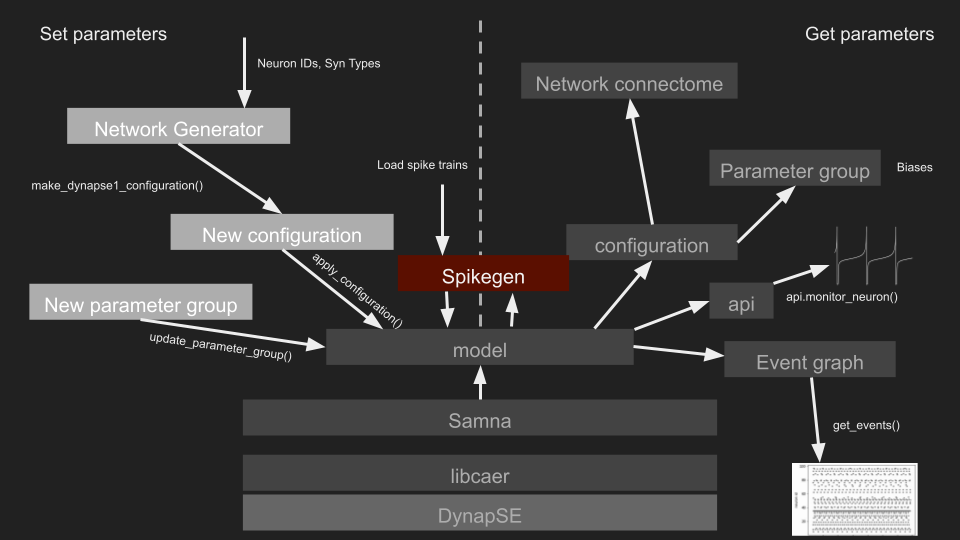
\includegraphics[width=\textwidth]{img/chapter4/Samna_architecture.png}
    \caption[Samna Python module architecture]{Architecture of the Samna Python package for interaction with the DYNAP-SE1 board~\cite{Samna}. The module provides an interactive \pyobject{model} object that supports four types of interactions:}
    \label{fig:enter-label}
\end{figure}

The architecture comprises an Interface class that holds the accessible state of the plasticity controller, such as the current values of the weight matrix, and provides the reward trigger function, while the Tracker class works in the background in a separate Python process, continuously fetching events from the chip in a loop with a set refresh rate and updating the values of the synapse trace variables.

For the presynaptic population of N neurons and the postsynaptic population of M neurons, the EPC creates an $N \times M$ array of virtual synapses and filters the spikes of the respective neurons in each pair.

The learning rule dictates that five state variables must be continuously updated for every synapse: $\{r_1, o_1, r_2, o_2, c\}$. The spike-triggered traces $\{r_1, o_1, r_2, o_2\}$, however, only depend on the activity of the respective neurons and can only be calculated once for every neuron instead of every synapse. The only state variable that is calculated for every pair of neurons is the eligibility trace $c(t)$.
This optimises memory resources and results in the scaling of the number of the state variables as $2(N+M)+N \times M$.

Another optimisation implemented in the R-STDP EPC is the event-driven (as opposed to clock-driven) update principle, so that the state variables $\{r_1, o_1, r_2, o_2, c\}$ are only updated at the moments of their access: either the spike on the pre- or postsynaptic neurons or the arrival of the reward for retrieving the current state of the eligibility traces. Since all of the traces are exponentially decaying, just by storing the last time of the trace update $t_{prev}$ and the trace value allows to retrieve the updated value on demand:

\begin{equation}
    f(t) = f(t_{prev})exp\left(-\frac{t-t_{prev}}{\tau}\right)
    \label{eq:relaxate}
\end{equation}

%\dz{ADD A TABLE OF ALL STATE VARIABLES}

\afterpage{
\begin{landscape}
\begin{figure}[h]
    \centering
    \captionsetup{width=1.6\textwidth}
    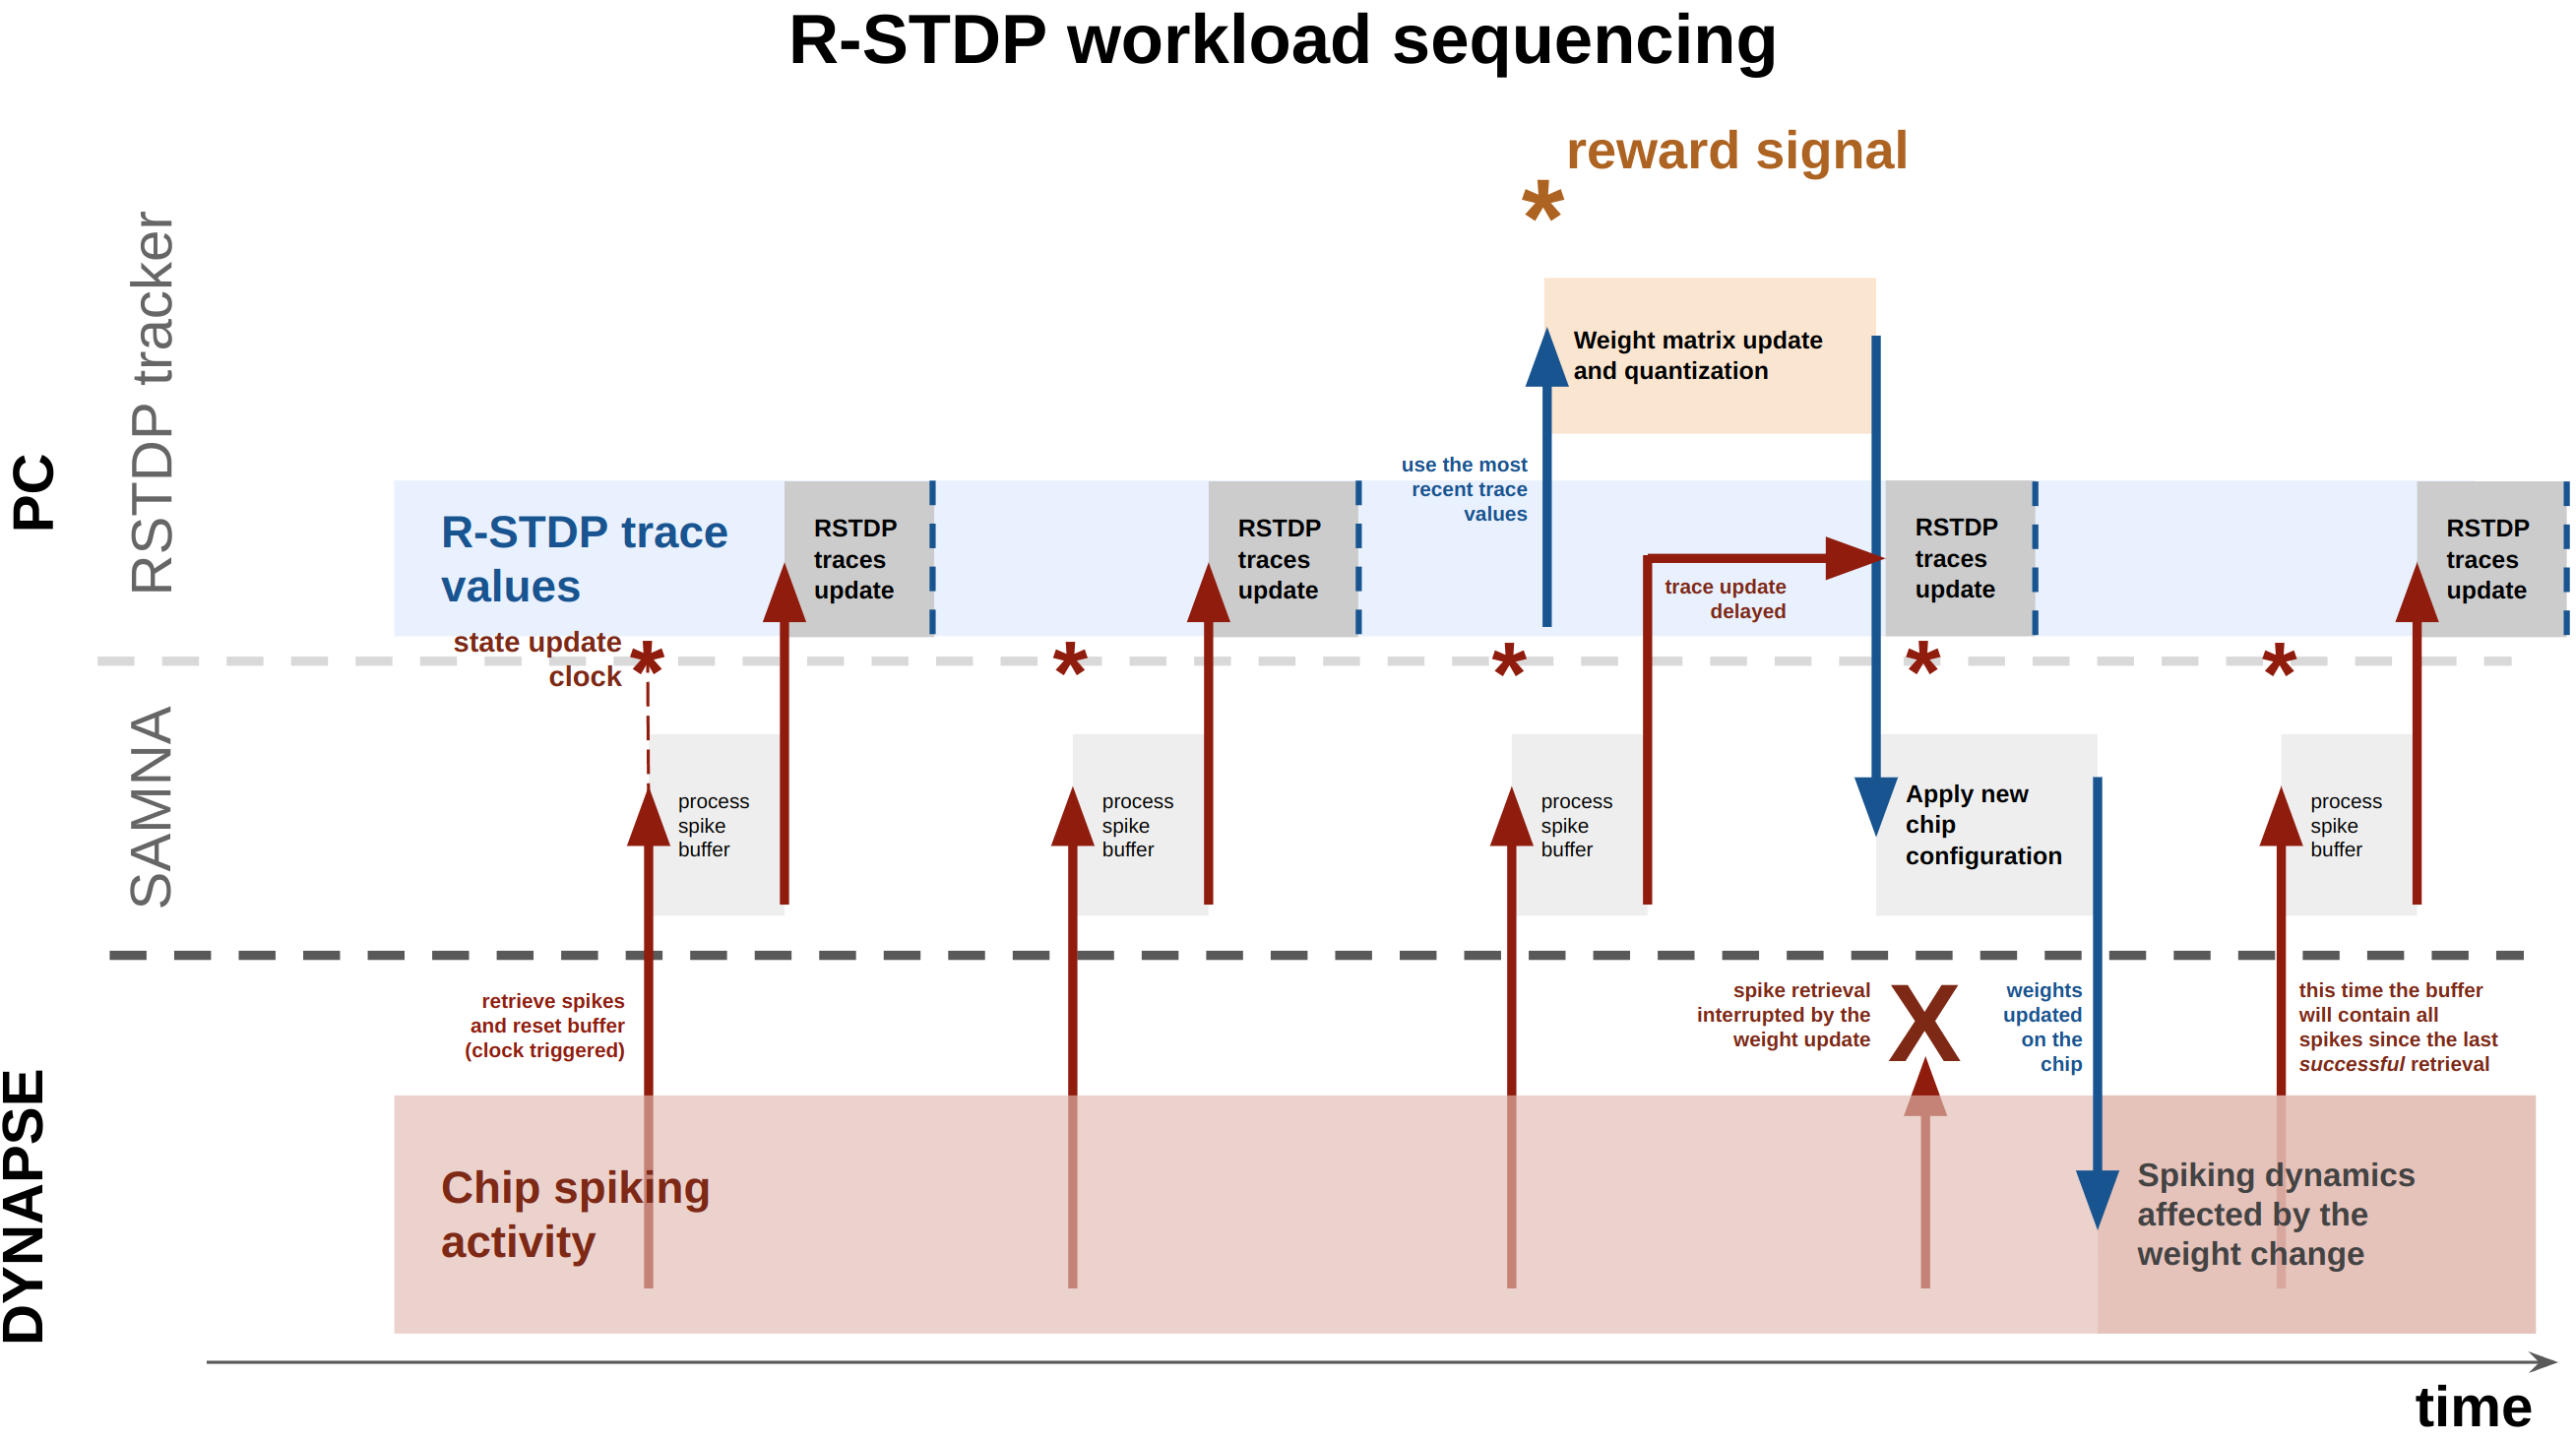
\includegraphics[width=1.5\textwidth]{img/chapter4/R_STDP_workload_sequencing.png}
    \caption[RSTDP algorithm DYNAP-SE1 with PC in the loop workload sequencing]{An illustration of the processing stages of the R-STDP algorithm with PC-in-the-loop implementation sequenced between the DYNAP-SE1 chip and parallel CPU processes. The chip provides neuronal dynamics (red) and outputs spikes that are collected to a buffer by the onboard FPGA. The Samna API has access to that buffer and can retrieve the spikes at any point in time, resetting the buffer to an empty state. The RSTDP tracker process uses a clock to make Samna periodically retrieve spikes and update all of the algorithm traces described by Eqs.~\ref{eq:ltp},~\ref{eq:ltd} and~\ref{eq:reward}. When the reward signal arrives, the calculation of the weight update starts immediately using the most recent values of the RSTDP traces, subsequently triggering Samna to perform the hardware weight update by reprogramming the spike router. Until the update is finished, the dynamics of the network assume the old state of the weight matrix, while the state is not retrieved. After the update finishes, the buffer is processed again normally, but including all of the spikes produced during the matrix update.}
    \label{fig:rstdp_workload_sequencing}
\end{figure}
\end{landscape}}


The interaction between the three parallel processes of the functioning EPC is shown in Figure~\ref{fig:rstdp_workload_sequencing}: the chip activity, the Samna filtering layer and the Tracker process. The Interface object receives updates from the Tracker at the same time the Tracker fetches events from Samna's event filters.



%\dz{ADD Trace update calcultaion} Only at discrete times!


%Dictionaries are used to ensure the access speed is uniform for every plastic synapse and does not depend on the 


%\dz{The reward is an instantaneous delta function instead of having some decaying concentration, meaning the weight, being a convolution of the reward and the eligibility trace, changes instantaneously by a fixed amount only, unlike the original paper.}

%\dz{benchmarking? time profiling?}


\subsection{Time precision limitations for the learning framework, time synchronization}

%\dz{Draw the diagrams for the FPGA processing of the frames}

%\dz{Discuss the FPGA clock synchronization issue:}
Any filters sorting on-chip spikes operate with asynchronous event timestamped by the onboard FPGA on DYNAP-SE1. The events are obtained through a buffered event filter that integrates them for some time. Even with the fast refresh rate, the time of processing the spikes in the Python API is delayed by one "frame". The third-factor input, or the reward signal, comes from the outside of the FPGA. Therefore, there is an inherent time mismatch for correct reward attribution.

On top of that, the application of the updated quantized matrix itself takes time. Specifically, the configuration update using Samna takes from 100 to 200ms to update, depending on the amount of changes in the matrix. The typical STDP coincidence detection window is 20-30ms, which means that setting for which our R-STDP framework is used must be adequate.

This imprecision, however, can be neglected if the system operates on long enough timescales and the individual STDP changes are small enough to only matter cumulatively when integrated by the eligibility traces.
%\dz{Reward delay is substantial for spiking timing but not in the scope of the timescales of behavioural tasks}


\section{Discussion}

The brain is asynchronous and saves resources on structural and communication expenses, and such are the considerations of the chip designers of the asynchronous neuromorphic boards. Remarkably, the constraints arising from those limitations have commonalities and similar solutions function in both domains.

For instance, let us take a look at the probabilistic rounding when quantizing the weights. The initial problem of low weight precision and fan-in constraint comes from considerations of saving the chip area, as for the example of the DYNAP-SE1 chip CAM cells each bit takes nine extra transistors~\cite{Pagiamtzis_Sheikholeslami06} and already take up more than 30\% of the area. For the same reason the analog circuits share configuration parameters as individual bias generators take substantial area as well if copied~\cite{Delbruck_etal10}. The working solution proposed in this chapter is to take advantage of the truly asynchronous nature of the chip routing scheme and program multiple CAM cells to subscribe to the same sender neuron address, scaling the postsynaptic current. The recruiting of the CAM cells proved to work best when done probabilistically, employing stochastic rounding. This principle (and its further development) can be mirrored with the biological counterpart of quantal neurotransmitter release~\cite{Redman90}, as in the neurotransmitters can be released in vesicles with a certain probability at a certain number of sites, resulting in ``quantal'' amplitudes of postsynaptic potentials. Thus, those observed postsynaptic potentials are also subject to variability between the activations, as well as the heterogeneity pattern dictated by the synaptic circuit evolution over its lifetime. In our case, the variability of PSPs in time would come through regular stochastic re-quantization of the weight matrix, leading to natural exploration. The fact that the brain robustly operates under similar principles gives us another reason to continue developing and embedding these strategies.

Another fitting consideration comes from the studies of using physical properties of materials in various ReRAM devices utilized as asynchronous synaptic elements~\cite{Covi_etal18, Covi_etal21, Dalgaty_etal24}, where the precision of individual weights might be low or drifting with time. If our online plasticity mechanisms keep fine-tuning the network's behaviour in a feedback loop keeping while being robust to those small changes, these hardware implementations would enable true low-power non-von Neumann edge computing.

A similar architecture approach to the one introduced in this chapter was taken by the team of BrainScales and their PPU unit that enables external plasticity for the chip~\cite{Pehle_etal22}. In both cases, it should be possible to exchange the equations to other learning rules quite seamlessly~\cite{Khacef_etal23}, having the same analog backend provide the spiking dynamics. An alternative to this kind of training is the adaptation of some pretrained network to the chip mismatch profile~\cite{Buchel_etal21}

Finally, the biological mechanism that came through naturally with the plasticity design route taken is structural plasticity. The nervous system is known to evolve over time and adapt to function it is tasked to perfect. The synapses are not only strengthened and weakened based on the activity, but also created and pruned~\cite{Spiess_etal16, George18}. In our framework, the EPC module, essentially, does not differentiate between the physically connected neurons and those that are not connected at the moment but whose activity might be correlated and which will have to be connected.

Perhaps future development of the EPC framework could include an extended version of structural plasticity. As filtering the spikes from too many neurons at once is still resource-heavy on the CPU, some strategy to selectively dynamically change the neurons from which the events are being filtered (thus reducing the amount of eligibility traces computed at once) could bring new interesting applications. This will make the framework more scalable for larger populations of neurons as well.

Another necessary design direction is improving the weight homeostasis rules~\cite{Muller_etal18a, George18}, including the quantization step optimisation. Given the interplay between the synaptic weight bias and the number of CAM slots used, an optimal balance should be possible to find.



%The idea for the implementation would be to create some \dz{Expand this.}\\\dz{check Richard George's work for references?}


%\dz{Applicability of quantization, batched weight updates approaches}

%\dz{brain connectivity is sparse, yet major reroutings are possible with plasticity}

%\dz{Put network mapping in this section or the previous chapter?}

%\dz{Discuss the ease of use of the other learning rules within the presented framework. Is batched update approach a prerequisite? Yes, because of the substantial time delay taken for application of the new connectivity matix.}

%\begin{figure}[h]
 % \centering
%    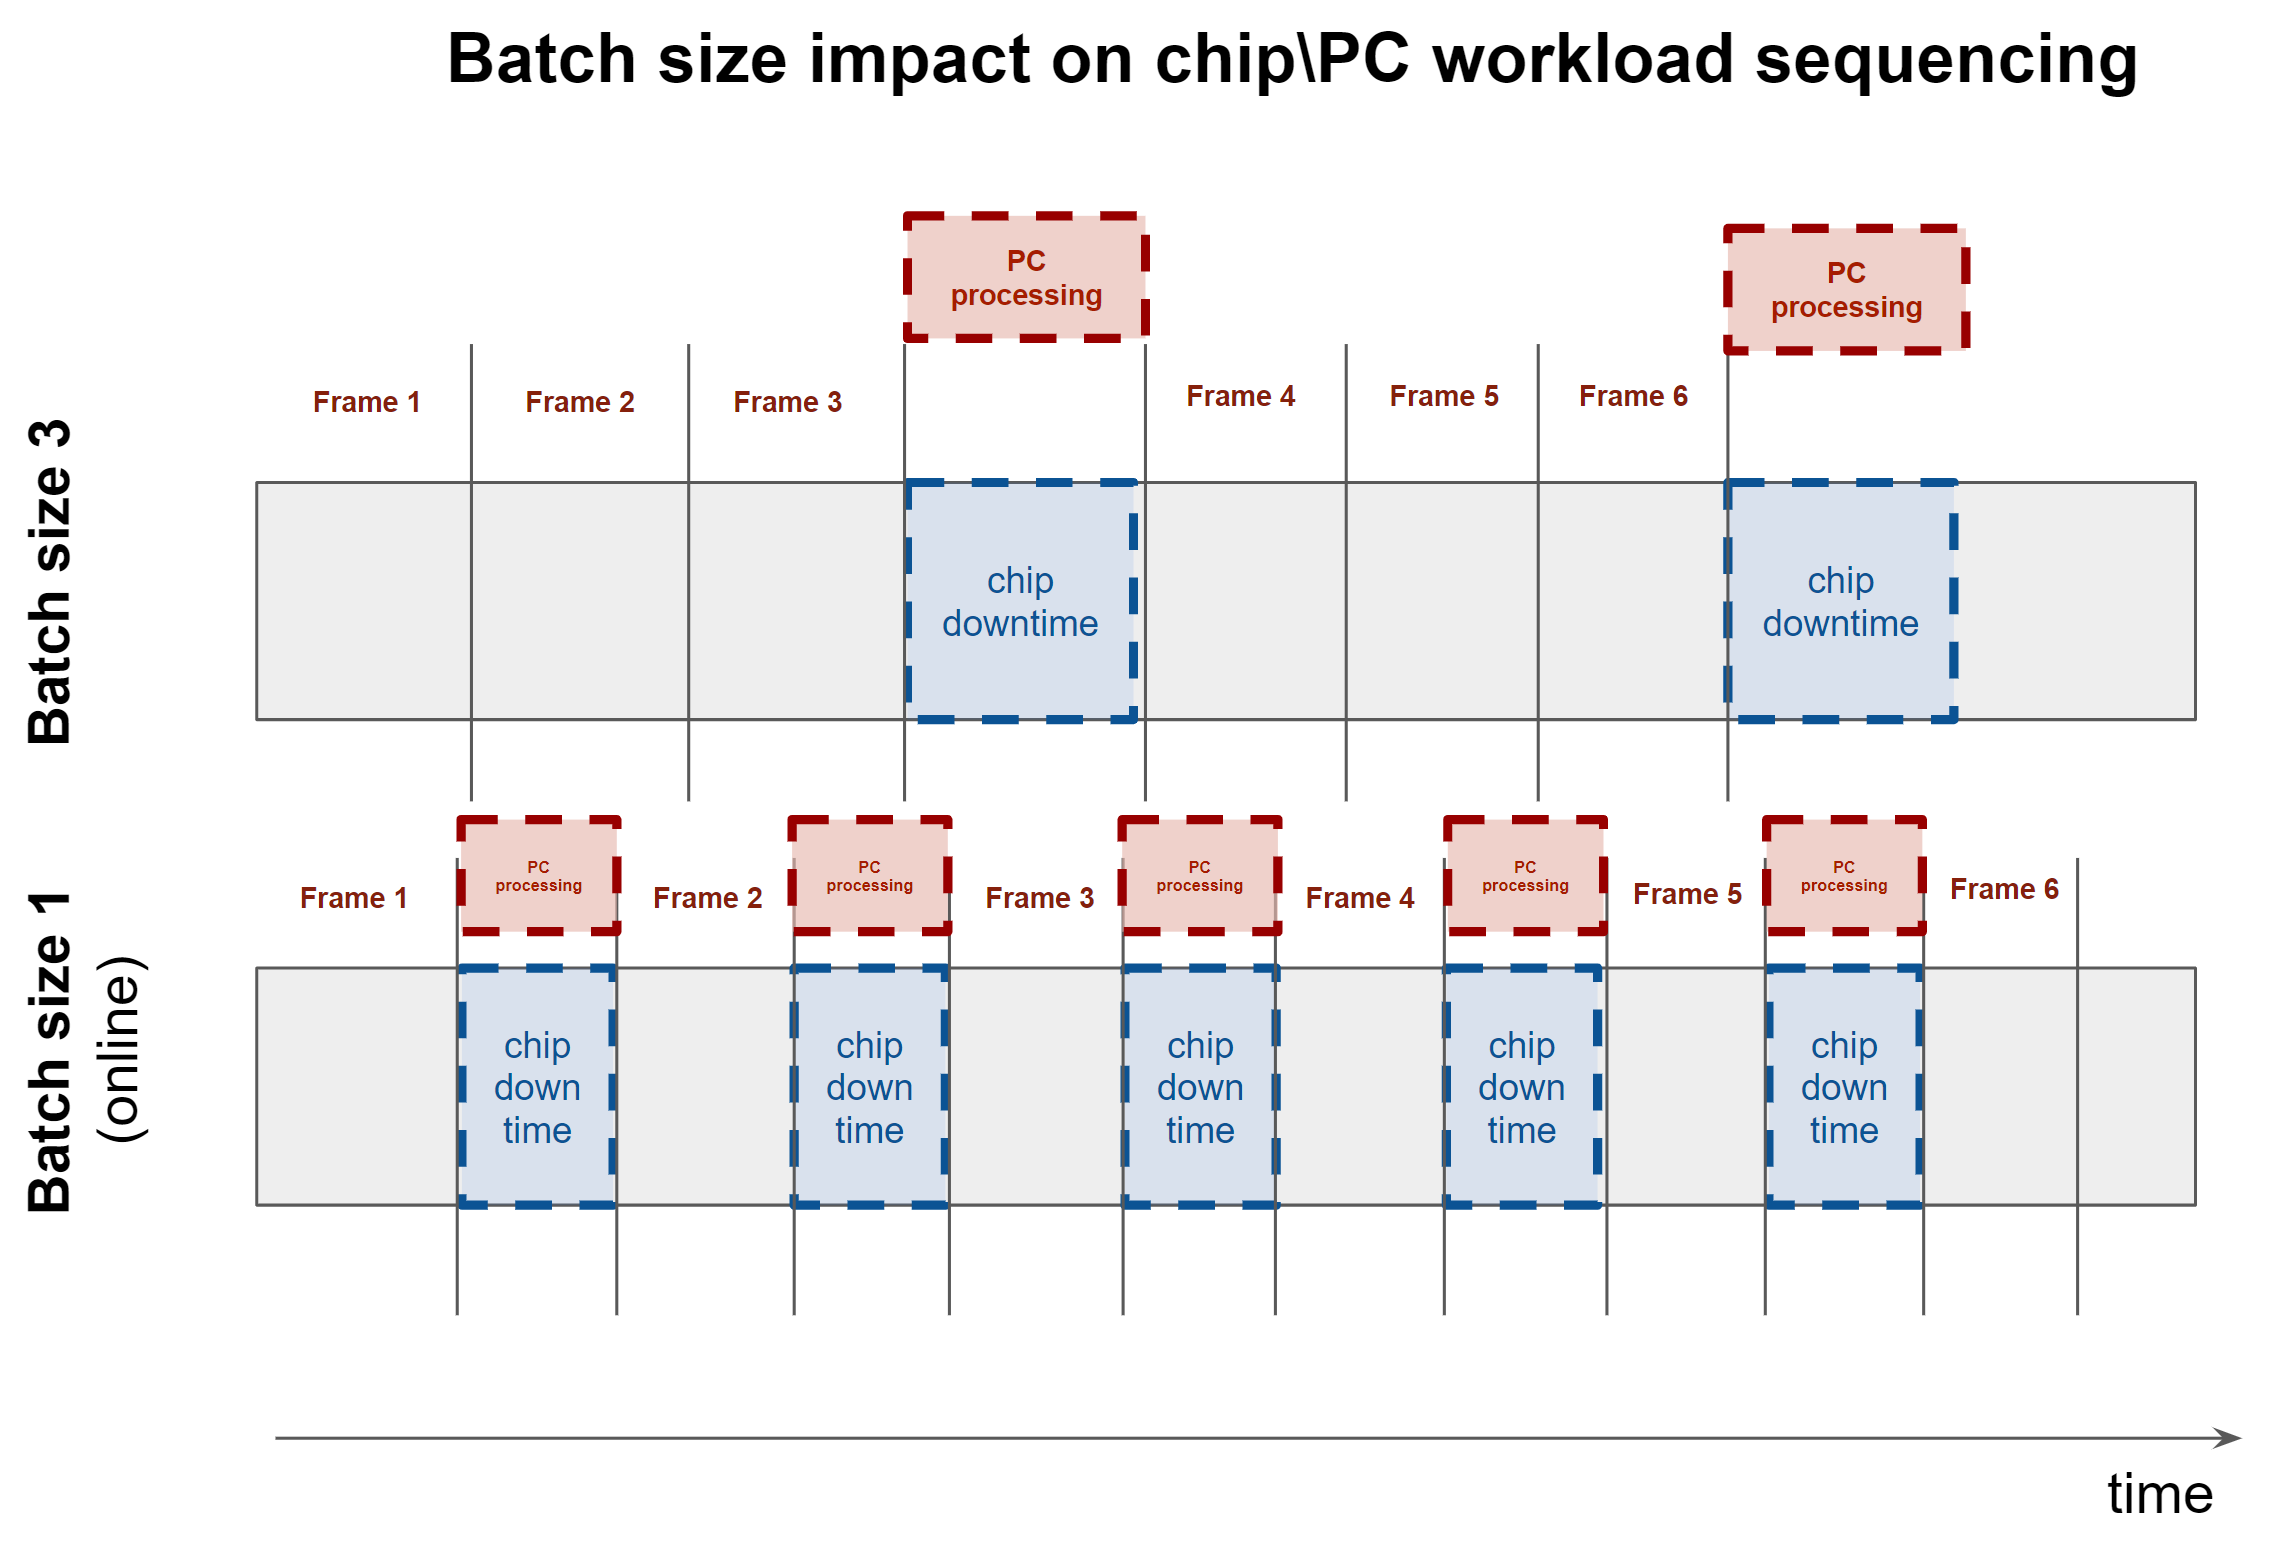
\includegraphics[width=.8\linewidth]{img/chapter5/batched_frame_processing.png}
 %   \caption[Batched frame processing approach for global chip interactions.]{Batched frame processing approach for global chip interactions case.}
%  \label{fig:batched_frame_processing}
%\end{figure}




%\section{Chip architecture}

%\dz{Very briefly introduce the analog/digital principle. Refer to the equations introduced in Chapter 2.}



%\section{Behaviour characterization: strategies and results}
%\label{section:chip_characterization}


%\subsection{Waveform capture and analysis}

%\dz{TBA: DPI equations and fitting waveforms using PyScope software}



%\subsection{Setting biases}





%\subsection{Mismatch and noise effects scaling}

%-- Introduce mismatch and noise as concepts


%\subsection{Constraints and their sources}

%-- Fan-in, fan-out
%-- CAM-clash

%\subsection{Achieving EI balance on the chip (?)}